\documentclass[12pt, a4paper, oneside]{report}             
\usepackage[czech]{babel}
\usepackage[backend=biber]{biblatex}
\addbibresource{citace.bib}
\usepackage[utf8]{inputenc}  
\usepackage{graphicx} % balíček pro vkládání RASTROVÝCH grafických souborů (PNG apod.)
%\usepackage{epsfig} % balíčky pro vkládání VEKTOROVÝCH grafických souborů typu EPS
%\usepackage{float} % rozšířené možnosti umístění obrázků
\usepackage{caption} % pro popisky obrázků, tabulek atd.

%\usepackage{tabularx} % rozšířené možnosti tabulek
%\usepackage{tabu} % jiný balík pro rozšířené možnosti tabulek
\usepackage{xcolor}
\usepackage{amsmath} % balíček pro pokročilou matematickou sazbu
%\usepackage{color} % pro možnost barevného textu
%\usepackage{fancybox} % umožňuje pokročilé rámečkování
%\usepackage{index} % nutno použít v případě tvorby rejstříku balíčkem makeindex
%\newindex{default}{idx}{ind}{Rejstřík} % zavádí rejstřík v případě použití balíku index
\usepackage[formats]{listings}  % Balíček pro sazbu zdrojových textů


\usepackage{anysize}
\marginsize{3.5cm}{1.5cm}{2.5cm}{3cm} % Nastavení okrajů (volitelné)

\usepackage{titlesec}  %přetypuje nadpisy všech úrovní na bezpatkové, tučné a dané velikosti

\titleformat{\chapter}[hang]{\sffamily\fontsize{16pt}{20pt}\bfseries}{\thechapter}{1em}{}
\titlespacing*{\chapter}{0pt}{20pt}{10pt}
\titleformat{\section}[hang]{\sffamily\fontsize{14pt}{16pt}\bfseries}{\thesection}{1em}{}
\titlespacing*{\section}{0pt}{20pt}{10pt}
\titleformat{\subsection}[hang]{\sffamily\fontsize{14pt}{18pt}\bfseries}{\thesubsection}{1em}{}
\titlespacing*{\subsection}{0pt}{20pt}{10pt}
\titleformat{\subsubsection}[hang]{\sffamily\fontsize{14pt}{18pt}\bfseries}{\thesubsubsection}{1em}{}
\titlespacing*{\subsubsection}{0pt}{20pt}{10pt}

\usepackage{setspace}
\setstretch{1.3} % Nastaví 1,3násobné řádkování

\frenchspacing % za větou bude mezislovní mezera (v anglických textech je mezera za větou delší)
\widowpenalty=1000 % "síla" zákazu vdov (= jeden řádek odstavce na konci stránky)
\clubpenalty=1000 % "síla" zákazu sirotků (= jeden řádek/slovo odstavce samostatně na začátku stránky)
\brokenpenalty=1000 % "síla" zákazu zlomu stránky za řádkem, který má na konci rozdělené slovo

\pagenumbering{arabic} % číslování stránek arabskými číslicemi
%\usepackage{fancyhdr} % Načte balíček pro pokročilé úpravy záhlaví a zápatí.
%\pagestyle{fancy} % Nastavení stylu stránek na 'fancy'
%\fancyhf{} % Vymazání aktuálního nastavení záhlaví a zápatí
%\fancyfoot[R]{\thepage} % Nastavení čísel stránek vpravo dole (R - right)
\makeatletter
  \renewcommand{\ps@plain}{\renewcommand{\@oddfoot}{\hfill\thepage} % Číslo stránky zarovnáno vpravo v zápatí
  \renewcommand{\@evenfoot}{\hfill\thepage} } % Pokud máte oboustranný dokument, zarovnání pro sudé stránky
\makeatother
\parindent=0pt % odsazení 1. řádku odstavce
\parskip=12pt   % mezera mezi odstavci
\usepackage[breaklinks=true,hypertexnames=false]{hyperref}  % Balíček 'hyperref' pro sazbu hypertextových odkazů. Hypertextové odkazy mohou obsahovat zalomení řádku. Názvy hypertext. odkazů budou tvořeny nezávisle na názvech TeXu.
\hypersetup{ % popisky v pdf souboru
  pdftitle={Systém chytré lednice "Easy Freezy"},    	% Pole 'Document Title'
  pdfauthor={Martin Robb},   	% Pole 'Author'
  pdfsubject={Kybernetika}, 						  	% Pole 'Subject'
  pdfkeywords={Klíčová slova}           	% Pole 'Keywords'
}

\usepackage{listings}
\usepackage{xcolor}

\definecolor{pycharm-green}{RGB}{87,166,74} % Comments
\definecolor{pycharm-blue}{RGB}{56,117,215} % Keywords
\definecolor{pycharm-orange}{RGB}{214,124,0} % Function names, decorators
\definecolor{pycharm-red}{RGB}{206,92,92} % Strings
\definecolor{pycharm-purple}{RGB}{170,85,255} % Built-in functions

\lstset{
    extendedchars=true,
    inputencoding=utf8,
    literate={á}{{'a}}1 {č}{{\v{c}}}1 {ď}{{\v{d}}}1 {é}{{'e}}1
             {ě}{{\v{e}}}1 {í}{{'i}}1 {ň}{{\v{n}}}1 {ó}{{'o}}1
             {ř}{{\v{r}}}1 {š}{{\v{s}}}1 {ť}{{\v{t}}}1 {ú}{{'u}}1
             {ů}{{\r{u}}}1 {ý}{{'y}}1 {ž}{{\v{z}}}1
             {Á}{{'A}}1 {Č}{{\v{C}}}1 {Ď}{{\v{D}}}1 {É}{{'E}}1
             {Ě}{{\v{E}}}1 {Í}{{'I}}1 {Ň}{{\v{N}}}1 {Ó}{{'O}}1
             {Ř}{{\v{R}}}1 {Š}{{\v{S}}}1 {Ť}{{\v{T}}}1 {Ú}{{'U}}1
             {Ů}{{\r{U}}}1 {Ý}{{'Y}}1 {Ž}{{\v{Z}}}1
}

%definice barev pythonu
\lstdefinestyle{python}{
    language=Python,
    commentstyle=\color{pycharm-green}, % Comments
    keywordstyle=\color{pycharm-blue}\bfseries, % Keywords
    stringstyle=\color{pycharm-red}, % Strings
    identifierstyle=\color{black}, % Variable names
    emph={self}, emphstyle=\color{pycharm-purple}, % Highlight 'self'
    morekeywords={True, False, None}, % Ensure booleans are highlighted
    basicstyle=\ttfamily, % Default text style
    tabsize=4, % Tab size
    showspaces=false,
    showstringspaces=false,
    breaklines=true
}

\bibliography{citace.bib}
%%%%%%%%%%%%%%%%%%%%%%%%%%%%%%%%%%%%%%%%%%%%%%%%%%%%%%%%%%%%%%%%%%%%%%%
%%%%%%%%%%%       Začátek dokumentu               %%%%%%%%%%%%%%%%%%%%%
%%%%%%%%%%%%%%%%%%%%%%%%%%%%%%%%%%%%%%%%%%%%%%%%%%%%%%%%%%%%%%%%%%%%%%%
\begin{document}
\thispagestyle{empty} %vypnutí číslování stránek

%% TITULNÍ STRANA %%%%%%%%%%%%%%%%%%%%%%%%%%%%%%%%%%%%%%%%%%%%%%%%%%%%%%%%%%%%%%
\begin{center}
  \begin{minipage}{3cm}
    
\includegraphics[width=2.86cm]{obrazky/logo.png}
  \end{minipage}
  \hfill
  \begin{minipage}{0.7\textwidth}
    \centering
    {\Large Vyšší odborná škola\\
    a Střední průmyslová škola elektrotechnická\\
    Plzeň, Koterovská 85\\ }
  \end{minipage}
  
  \vspace{2cm}
  %% VYBERTE TYP PRÁCE %%%%%%%%%%%%%%%%%%%%%%%%%%
  {\Large \textbf{DLOUHODOBÁ MATURITNÍ PRÁCE S~OBHAJOBOU}\\ }
  % {\Large \textbf{ROČNÍKOVÁ PRÁCE}\\ }
  %%%%%%%%%%%%%%%%%%%%%%%%%%%%%%%%%%%%%%%%%%%%%%%
  
  \vspace{2.5cm}
  {\large Téma: \\ }
  \vspace{0.25cm}
  %% PŘEPIŠTE NÁZEV PRÁCE %%%%%%%%%%%%%%%%%%%%%%%%%%%
  {\LARGE \textbf{Systém chytré ledničky "Easy Freezy"}}  
  %%%%%%%%%%%%%%%%%%%%%%%%%%%%%%%%%%%
  
  \vfill
\end{center}
\begin{tabular}{{p{4.5cm} p{12cm}}}
  {\Large \textbf{Autor práce:}} & \Large{Martin Robb} \\
  {\Large \textbf{Třída:}} & \Large{4.L} \\ 
  {\Large \textbf{Vedoucí práce:}} & \Large{Ing. Pavel Jedlička} \\ 
  {\Large \textbf{Dne:}} & \Large{1.1.2030} \\ 
  {\Large \textbf{Hodnocení:}} &  \\ 
\end{tabular}
%% Vložení zadání %%%%%%%%%%%%%%%%%%%%%%%%%%%%%%%%%%%%%%%%%%%%%%%%%%%%%%%%%%%%
\newpage
\thispagestyle{empty}
%\includepdf[pages=1]{pdf/student-zadani}% název souboru nesmí obsahovat mezery!
%% NEBO lze vytvořit prázdný list příkazem ze šablony
\vspace{4cm}
{\sffamily\Huge\centering ZDE VLOŽIT LIST ZADÁNÍ}

{\sffamily\centering Z~důvodu správného číslování stránek}
%\newpage   % při dvojstranném tisku se přidá prázdná stránka

%%%%%%%%%%%% Anotace a poděkování %%%%%%%%%%%%%%%%%%%%%%%%%%%%%%%%%%%%%%%%%%%%%%
\newpage
\chapter*{Anotace a poděkování} \indent
\thispagestyle{empty}
Maturitní práce se zabývá vývojem mobilní aplikace pro Android, která organizuje domácí zásoby potravin. Aplikace skenuje čárový kód a datum spotřeby produktu. Dále najde informace produktu pomocí naskenovaných dat v externí databázi potravin (Open Food Facts). Získané informace následně ukládá do databáze. Aplikace umožňuje uživateli tuto databázi  upravovat.

\vfill

Prohlašuji, že jsem tuto práci vypracoval samostatně a použil literárních pramenů a~\mbox{informací}, které cituji a uvádím v seznamu použité literatury a zdrojů informací.

Prohlašuji, že jsem nástroje UI využil v souladu s principy akademické integrity a že na využití těchto nástrojů v práci vhodným způsobem odkazuji.

Souhlasím s využitím mé práce učiteli VOŠ a SPŠE Plzeň k výuce.

\vspace{1cm}

V Plzni dne 1. 1. 2030 \hfill Podpis: ..........................

%%%%%%%%%%%% Obsah práce ... je generován AUTOMATICKY %%%%%%%%%%%%
\newpage
\tableofcontents
\thispagestyle{empty}

%--------------------------------------------------------
%|         Zde začíná SAMOTNÁ PRÁCE (text)              |
%--------------------------------------------------------
\newpage

\chapter*{Úvod}
\addcontentsline{toc}{chapter}{Úvod}
%uvod do prace neco jako anotace ale trochu delsi
\section*{Motivace}
Aplikací, které napodobují chytrou lednici není mnoho. Zároveň také popularita chytrých ledniček rok od roku vzrůstá. V této práci jsem se chtěl pokusit o napodobení těchto chytrých lednic bez toho aby uživatel musel tyto drahé a prostor zabírající lednice kupovat. Pokusím se hlavně napodobit databázový systém produktů a expiračních dat, práce a~upravování dat v databázi z uživatelského rozhraní (dále jen UI) i samotné zobrazování dat produktů z databáze.

\section*{Výběr programovacího jazyku}
Pro realizaci aplikace jsem se rozhodl využít programovací jazyk Python \cite{python}. Hlavním důvodem tohoto rozhodnutí je skutečnost, že Python je jediným jazykem který znám. Jako ideální jazyky pro vývoj aplikací pro Android je často uváděn jazyk Java nebo Kotlin. Python sice uváděn není pro vývoj Android aplikací ho ale použít lze. Musíme však využít vhodný framework, který se postará o kompatibilitu s Androidem.

\section*{Kivy}
Kivy je vývojová platforma pro jazyk Python, která se je využívaná pro vývoj aplikací na Android, IOS ale i Windows. Existuje ještě alternativní vývojová platforma BeeWare, která je ještě v rané fázi vývoje a proto také méně používaná. Kivy je proto momentálně nejlepší volbou pro vývoj aplikace na Android pomocí Pythonu. Dále také používám KivyMD. KivyMD je rozšíření frameworku Kivy, které usnadňuje úpravy a vytváření grafického rozhraní aplikace.
\chapter{Získávání dat o produktech}
Je nutné uvědomit si jaké data o produktech je potřeba. Je potřeba datum expirace a~čárový kód produktu. Čárový kód umožňuje dohledání dalších informací v externí databázi jako například jméno, výrobce nebo také ale počet kalorii na 100g atd. Já využívám veřejně dostupnou databázi OpenFoodFacts \cite{openfoodfacts}. Pro mé účely stačí jen jméno produktu.
Nejdříve jsem plánoval stáhnout obsah celé přístupné databáze. Naskytla se ale mnohem lepší varianta. OpenFoodFacts podporují získávání dat přímo z jejich webových stránek. Stačí tedy zadat určitou URL adresu, která obsahuje čárový kód daného produktu, do vyhledávání a jako odpověď získáme JSON soubor s informacemi o daném produktu viz Listing \ref{ziskavani_dat_produktu}. 

\begin{lstlisting}[style=python,label=ziskavani_dat_produktu,caption=Ukázka získání JSON souboru produktu]
url = f"https://world.openfoodfacts.org/api/v2/product/{carovy_kod}.json"
odpoved = requests.get(url)
odpoved_json = odpoved.json()
 produkt_api_data = api_json_file.get("product", "Unknown")
}
\end{lstlisting}
Na začátku vloženého ukázkového programu (viz Listing 1.1 \ref{ziskavani_dat_produktu}) lze vidět string (posloupnost textových charakterů) pojmenovaný "url". Do tohoto stringu je vložen čárový kód mezi složené závorky. Dále je využita knihovna Requests \cite{requests}, která umožňuje vyhledávání, získání odpovědi serveru a následné převedení (přeparsování) na formát JSON. Do proměnné "response" se uloží odpověď serveru na poslanou URL a následně se ukládá přeparsovaná verze odpovědi do proměnné "odpoved\_json". V posledním řádku se z této odpovědi získávají všechny informace o produktu a ukládají do proměnné "produkt\_api\_data". Jednotlivé informace se dále získávají z proměnné "produkt\_api\_data" ~stejným způsobem.

\section{Kalendář}
Pro získání data expirace produktu jsem se rozhodl použít kalendář. Uvažoval jsem, že bych mohl využít kamery zařízení pro naskenovaní data expirace. Kvůli tečkovanému tisku dat expirace a lesklému obalu byla ale často nepřesná a tak jsem se od tohoto nápadu odklonil. Rozšíření KivyMD \cite{kivymd} již v sobě jistý kalendář (anglicky datepicker) pro výběr dat obsahuje, bohužel ale nepodporuje některé funkce, které chci aby kalendář měl jako například vybrání více dat spotřeby. Rozhodl jsem se tedy zkonstruovat vlastní.

Kalendář je rozdělen na několik sekcí. Každá z těchto sekcí má jinou náležitou funkci. Sekce popisuji podle obrázku \ref{fig:datepickerSekce}. Nejdříve je 1. vrstva  popisek, který zobrazuje rok a měsíc, ve kterém vybíráme datum. Pod touto sekcí jsou tlačítka, které slouží pro změnu měsíce V další sekci každé tlačítko představuje jednotlivé dny v měsíci. V poslední sekci jsou umístěna tlačítka pro uložení nebo pro zrušení výběru a následné ukončení aplikace. Výsledný kalendář je zachycen na Obrázku \ref{fig:datepicker}.

Hlavní část kalendáře jsou tlačítka pro výběr jednotlivých dnů v měsíci (na Obrázku \ref{fig:datepickerSekce} označeno číslem 4). Počet těchto tlačítek se musí přizpůsobit podle toho v jakém měsíci uživatel právě vybírá. Proto kalendář vždy musí smazat předchozí a vygenerovat nové tlačítka když uživatel stiskne jedno ze dvou tlačítek pro změnu měsíce (na Obrázku \ref{fig:datepickerSekce} označeno číslem 2). Funkce tlačítek je znázorněna v podobě diagramu na obrázku \ref{fig:changeDateDiag}.
%ještě bych možná přidal jak se to ukončuje???

\begin{figure}[t!]
    \centering
    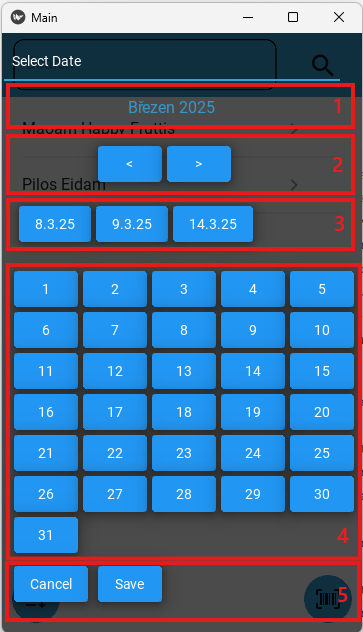
\includegraphics[width=0.4\linewidth]{obrazky/datepickerUpraveneNaSekce.png}
    \caption{Kalendář rozdělený na jednotlivé sekce}
    \label{fig:datepickerSekce}
\end{figure}

%rozhodni se jestli to tu nechat nebo použít jen ten rozdělený na sekce
\begin{figure}[b!]
    \centering
    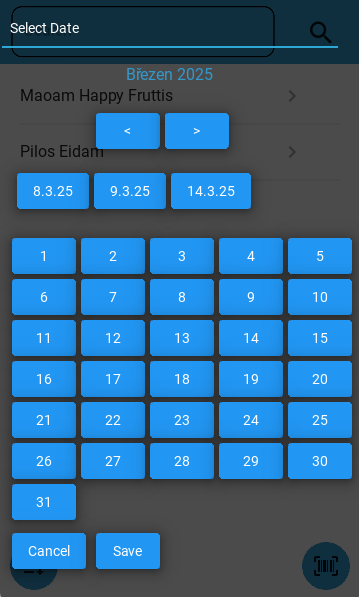
\includegraphics[width=0.4\linewidth]{obrazky/datepicker.png}
    \caption{Kalendář}
    \label{fig:datepicker}
\end{figure}

\begin{figure}
    \centering
    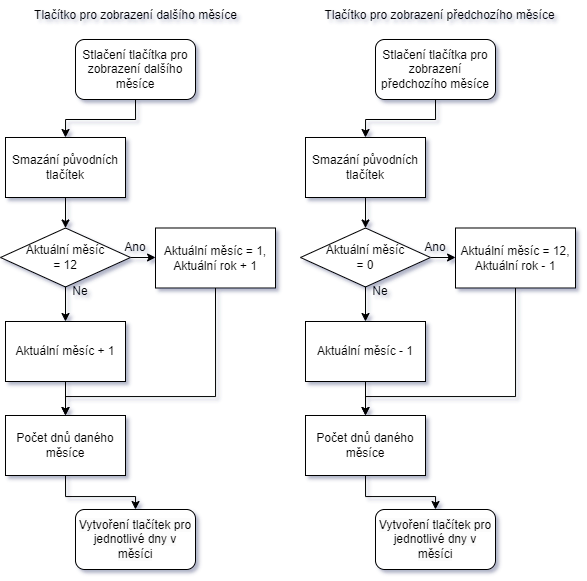
\includegraphics[width=0.6\linewidth]{obrazky/change_date.png}
    \caption{Diagram změny měsíce}
    \label{fig:changeDateDiag}
\end{figure}
\clearpage

\section{Čtení čárového kódu}
%jak to dělam
%ukázat část kódu
%diagram
\chapter{Databáze}
%popiš proč používám MYSQL (jsem idiot),
\section{Uživatelská databáze}
%ukaž strukturu, screenshot z workbenche a proč používám Varchar (taky protože jsem idiot)
\section{Komunikace s databází}
%co používám pro komunikaci s datab., ukaž kód  
\begin{lstlisting}[style=python]
class Content(MDBoxLayout):
    def __init__(self, items, id, product_container, **kwargs):
        #zdedeni parametru materske tridy
        super().__init__(**kwargs)

        self.orientation = "vertical"
        self.size_hint_y = None
        self.id = id
        self.product_container = product_container

        # prizpusobeni vysky podle poctu dat expirace
        self.dates_array = items
        self.items = len(items)
        self.height = dp(35 * self.items) #old dp 48

}
\end{lstlisting}
\chapter{Aplikace na Android}

\section{Hlavní aplikace}

\begin{lstlisting}[style=python]
class Content(MDBoxLayout):
    def __init__(self, items, id, product_container, **kwargs):
        #zdedeni parametru materske tridy
        super().__init__(**kwargs)

        self.orientation = "vertical"
        self.size_hint_y = None
        self.id = id
        self.product_container = product_container

        # prizpusobeni vysky podle poctu dat expirace
        self.dates_array = items
        self.items = len(items)
        self.height = dp(35 * self.items) #old dp 48

}
\end{lstlisting}

\clearpage

\subsection{Seznam použitých knihoven, frameworků a nástrojů}
\begin{itemize}
    \item OpenCV (CV2) \cite{opencv}
    \item Ubuntu \cite{ubuntu}
    \item KivyMD \cite{kivymd}
    \item MYSQL connector \cite{mysql-connector}
    \item Collections \cite{python-collections}
    \item Datetime \cite{python-datetime}
    \item Buildozer \cite{buildozer}
    \item Python \cite{python}
    \item Requests \cite{requests}
    \item Kivy \cite{kivy}
\end{itemize}

\chapter*{Závěr}
\addcontentsline{toc}{chapter}{Závěr}
Tolik k rychlému úvodu a ukázce. Tento template by měl být rovnou použitelný pro vaši práci. Pouze upravíte titulní stránku a text v práci. Níže je ještě použitá literatura. Pokud byste měli nějaké dotazy, zkuste google (latex je velice dobře komunitně podporován a najdete odpovědi na všechny problémy online). Případně se obraťte na autora dokumentu.

% CITACE ---------------------------------------------------------------------------
\printbibliography
% konec citací
% Přílohy: 
%\chapter*{Přílohy}
%\pagenumbering{Roman}
%\addcontentsline{toc}{chapter}{Přílohy}
\end{document}